\section{한국 5G 특화망조사}
\subsection{5G 특화망이란?}
5G는 5세대 이동통신을 뜻하며 최대 속도가 20Gbps에 달하는 최신 이동통신 기술,기존의 3개 통신사업자만이 전용주파수를 할당받아 전국을 대상으로 대규모 네트워크를 구축하여 대국민 서비를 제공하는 기존의 5g 네트워크와 대비해서 5g 특화망은 이동통신 전용 상용망 이외의 주파수를 이용해서 특정공간 (건물, 시설, 장소) 등에서 수요기업이 도입하고자 하는 네트워크를 구축하는 사용자화 네트워크이다.  

수요기업은 행정적 신청절차를 통해 4.7GHz, 28GHz 대역의 특화망 주파수를 지정 할당받아 필요에 다른 네트환경을 구축할 수 있다.\\
    \vspace{-4mm}
    \begin{figure}[!h]\centering
		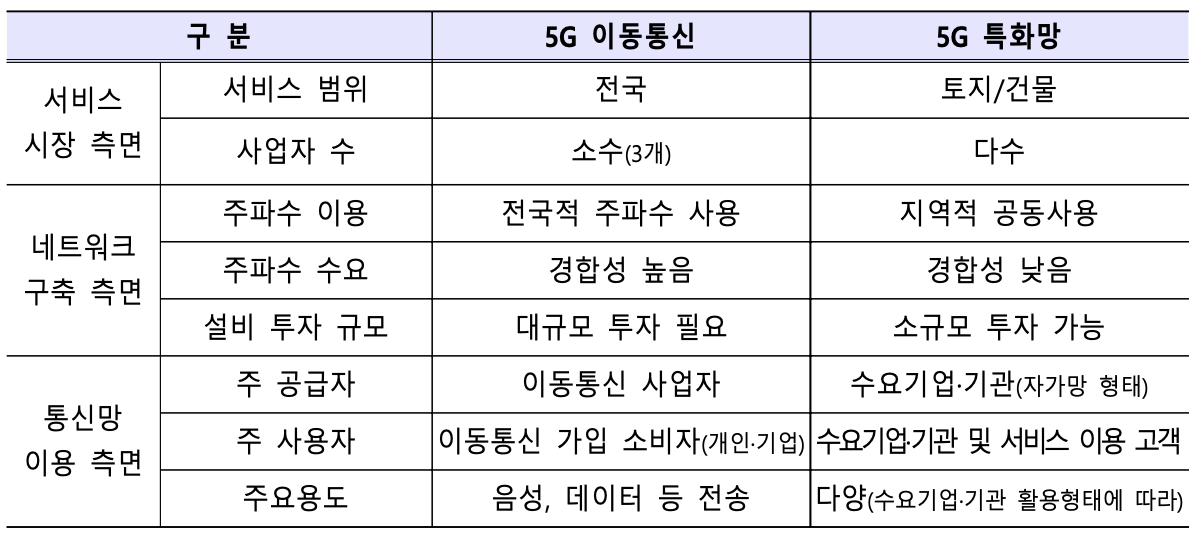
\includegraphics[width=.75\textwidth]{image/week03/2-1.png}
		\caption{\small 5G 이동통신과 특화망의 비교}
		\vspace{-10pt}
    \end{figure}
% \subsubsection*{5G 네트워크의 구성}
% \subsubsection*{5G 특화망}
\clearpage
\subsection{국내 5G 특화망, 이음 5G 현황}
기존 ‘5G 특화망’ 이라는 이름으로 사용되었지만, 작년말 이음 5G의 명칭으로 변경되었다. 
\subsubsection*{이음 5G 시장 참여자의 유형}
    \begin{figure}[!h]\centering
		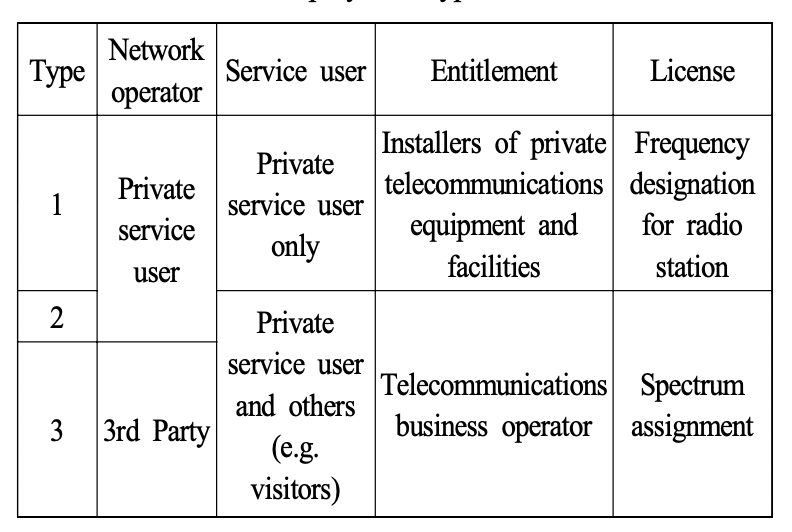
\includegraphics[width=.65\textwidth]{image/week03/2-2-1.png}
		\caption{\small 5G 이동통신과 특화망의 비교}
		\vspace{-10pt}
    \end{figure}
\subsubsection*{한국 이음 5G의 주파수 배치}
    \begin{figure}[!h]\centering
		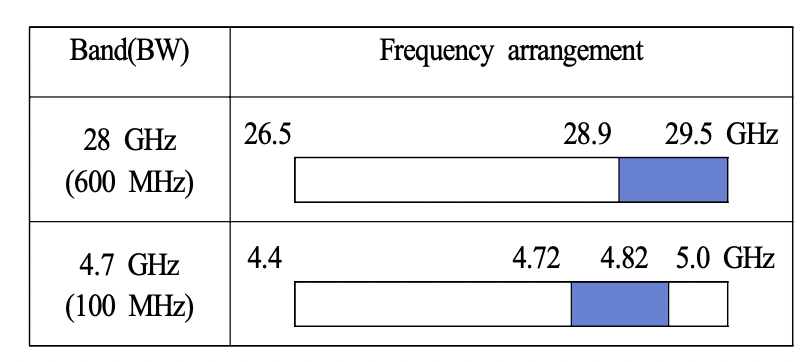
\includegraphics[width=.65\textwidth]{image/week03/2-2-2.png}
		\caption{\small 5G 이동통신과 특화망의 비교}
		\vspace{-10pt}
    \end{figure}
% \subsubsection*{네트워크 기반실설의 기술수준}
%     \begin{figure}[!h]\centering
% 		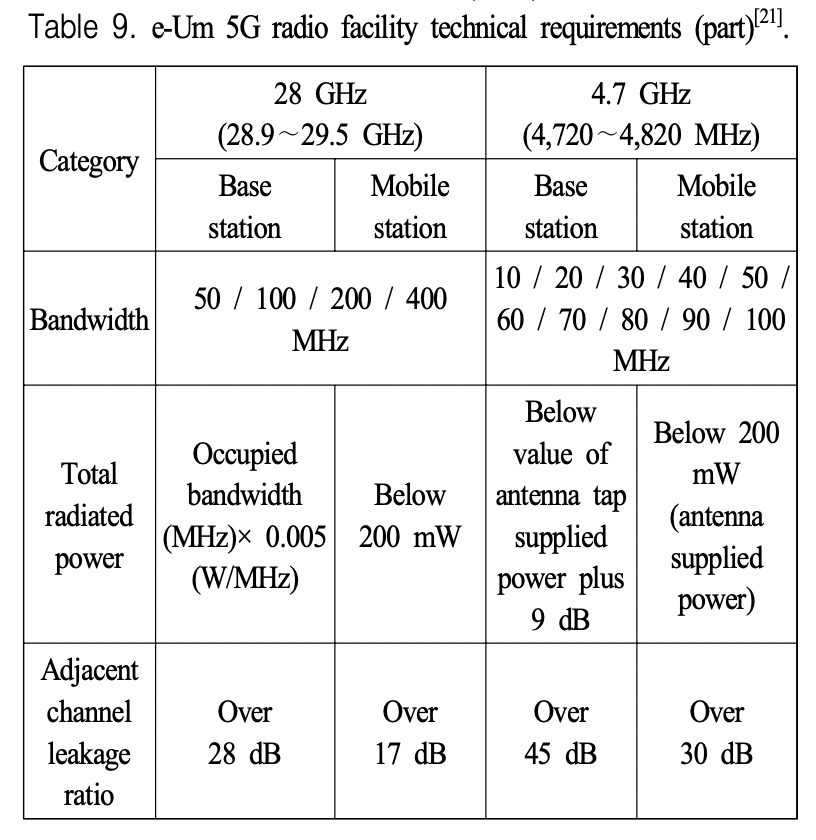
\includegraphics[width=.65\textwidth]{image/week03/2-2-3.png}
% 		\caption{\small 5G 이동통신과 특화망의 비교}
% 		\vspace{-10pt}
%     \end{figure}